\section{Evaluation}
\label{sec:validation}

In this section we present the validation of our approach. As aforementioned, this validation is twofold. On one hand, we demonstrate that our approach is correct. To do so, we take use a case study that is well documented in \cite{Crane:2007} and where we exactly know the commonalities existing among the input set. We execute our approach and we compare the result. The second part of the evaluation corresponds to demonstrate that our approach is relevant. That is, we demonstrate with empirical data that the phenomenon of syntactic and semantic commonalities is currently appearing in real DSLs and, so, our approach is relevant. 

\subsection{Evaluating correctness: The state machines case study}

The case study is composed of three different DSLs for expressing state machines: UML state diagrams, Rhapsody, and Harel's state charts. Because the three DSLs are intended to express the same formalism, they have commonalities. For example, all of them provide the basic concepts of State and Transition. However, not all those DSLs are exactly the same. In fact, they have some syntactic and semantic differences. As an example of syntactic particularities consider the case of the pseudostates. As an example of semantic differences consider the case of ... Whereas... 

\subsubsection{The oracle.} We are interested on this case study because it corresponds to a set of DSLs where the commonalities and differences are quite well documented. Hence, if we implement those DSLs by strictly following such documentation, we have an oracle to test the correctness of our approach. 

\begin{figure}
\centering
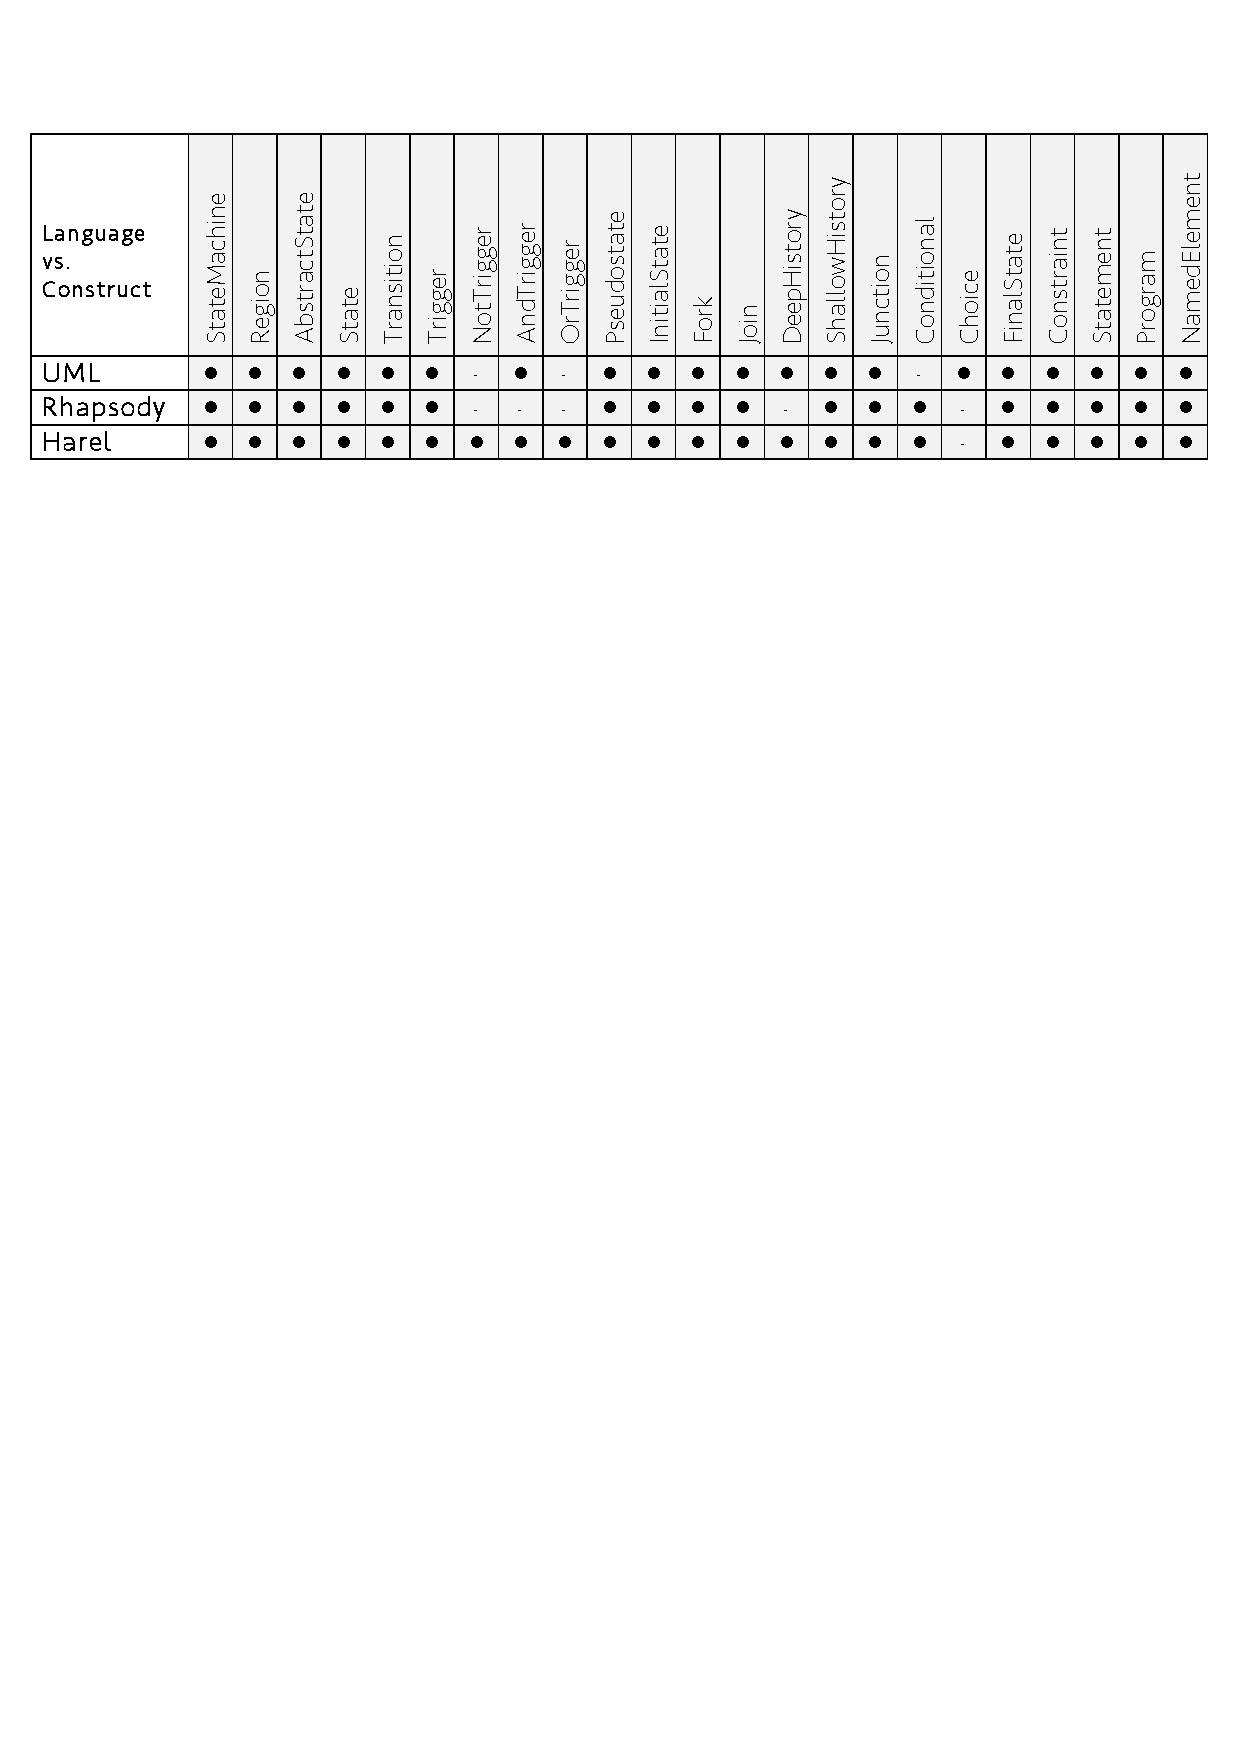
\includegraphics[width=1\linewidth]{images/oracle.pdf}
\caption{Oracle for evaluation of correctness}
\label{fig:oracle}
\end{figure}

Figure \ref{fig:oracle} shows a table with the constructs contained in the case study. Not all the DSLs have exactly the same constructs. For example, while constructs such as StateMachine, Region, State, and Transitions are shared by all the DSLs, the peudostates, the triggers, are different for each case. 

\subsubsection{Results.} The figure \ref{fig:puzzle-overlapping} shows the results of the first part of the analysis performed by our approach. It presents the Venn diagram produced for the case study of the state machines. As you can see at the left, the numbers correspond to the oracle presented in table X. The case of the semantics is revealing as well. 

\begin{figure}
\centering
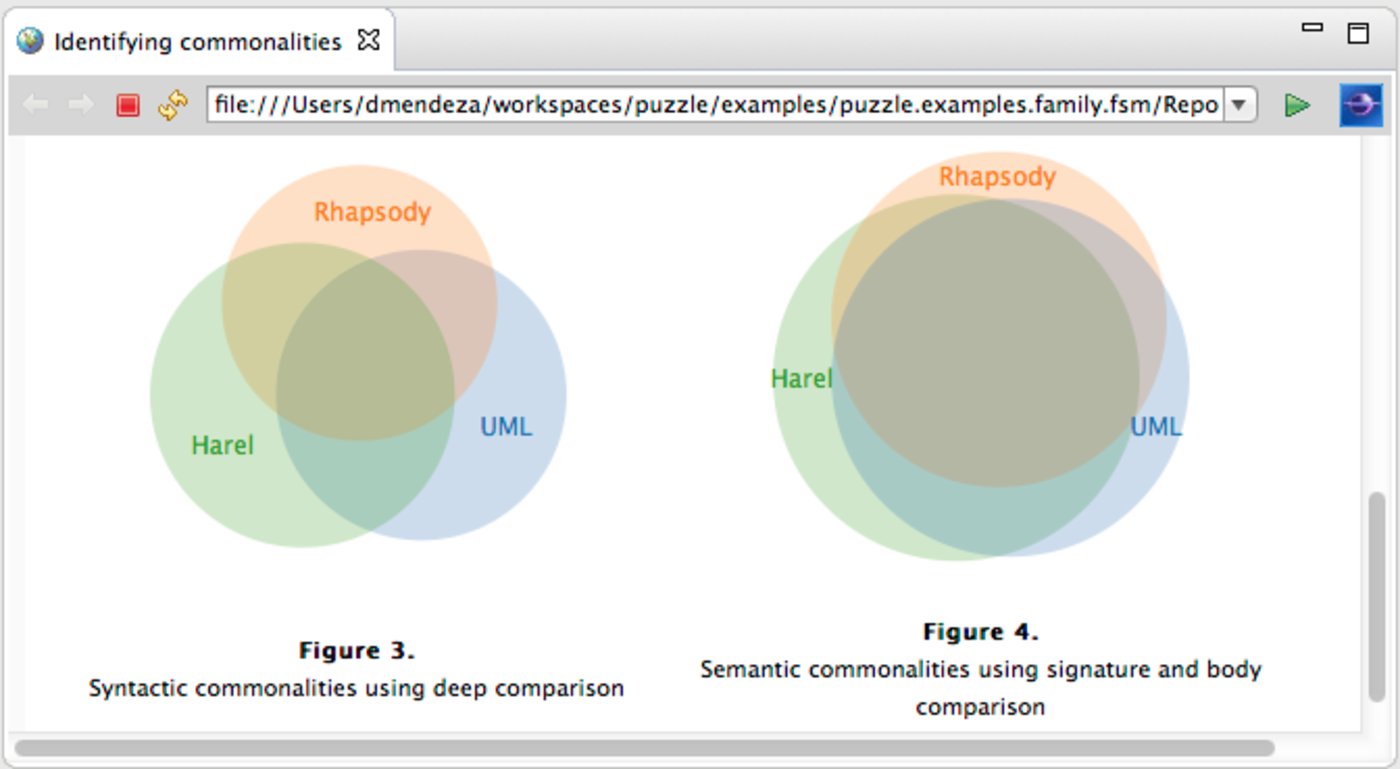
\includegraphics[width=1\linewidth]{images/puzzle-overlapping.pdf}
\caption{Results for the state machines case study: identifying overlapping}
\label{fig:puzzle-overlapping}
\end{figure}

In turn, Figure \ref{fig:puzzle-modularization} shows the results for the second  and third part of the approach: identifying and extracting reusable language modules. As the reader may expect, there is a core module that contains all those language constructs that are shared by the three DSLs i.e., the intersection of the three DSLs. Then, the reusable language modules regard the pseudostates and the triggers.

\begin{figure}
\centering
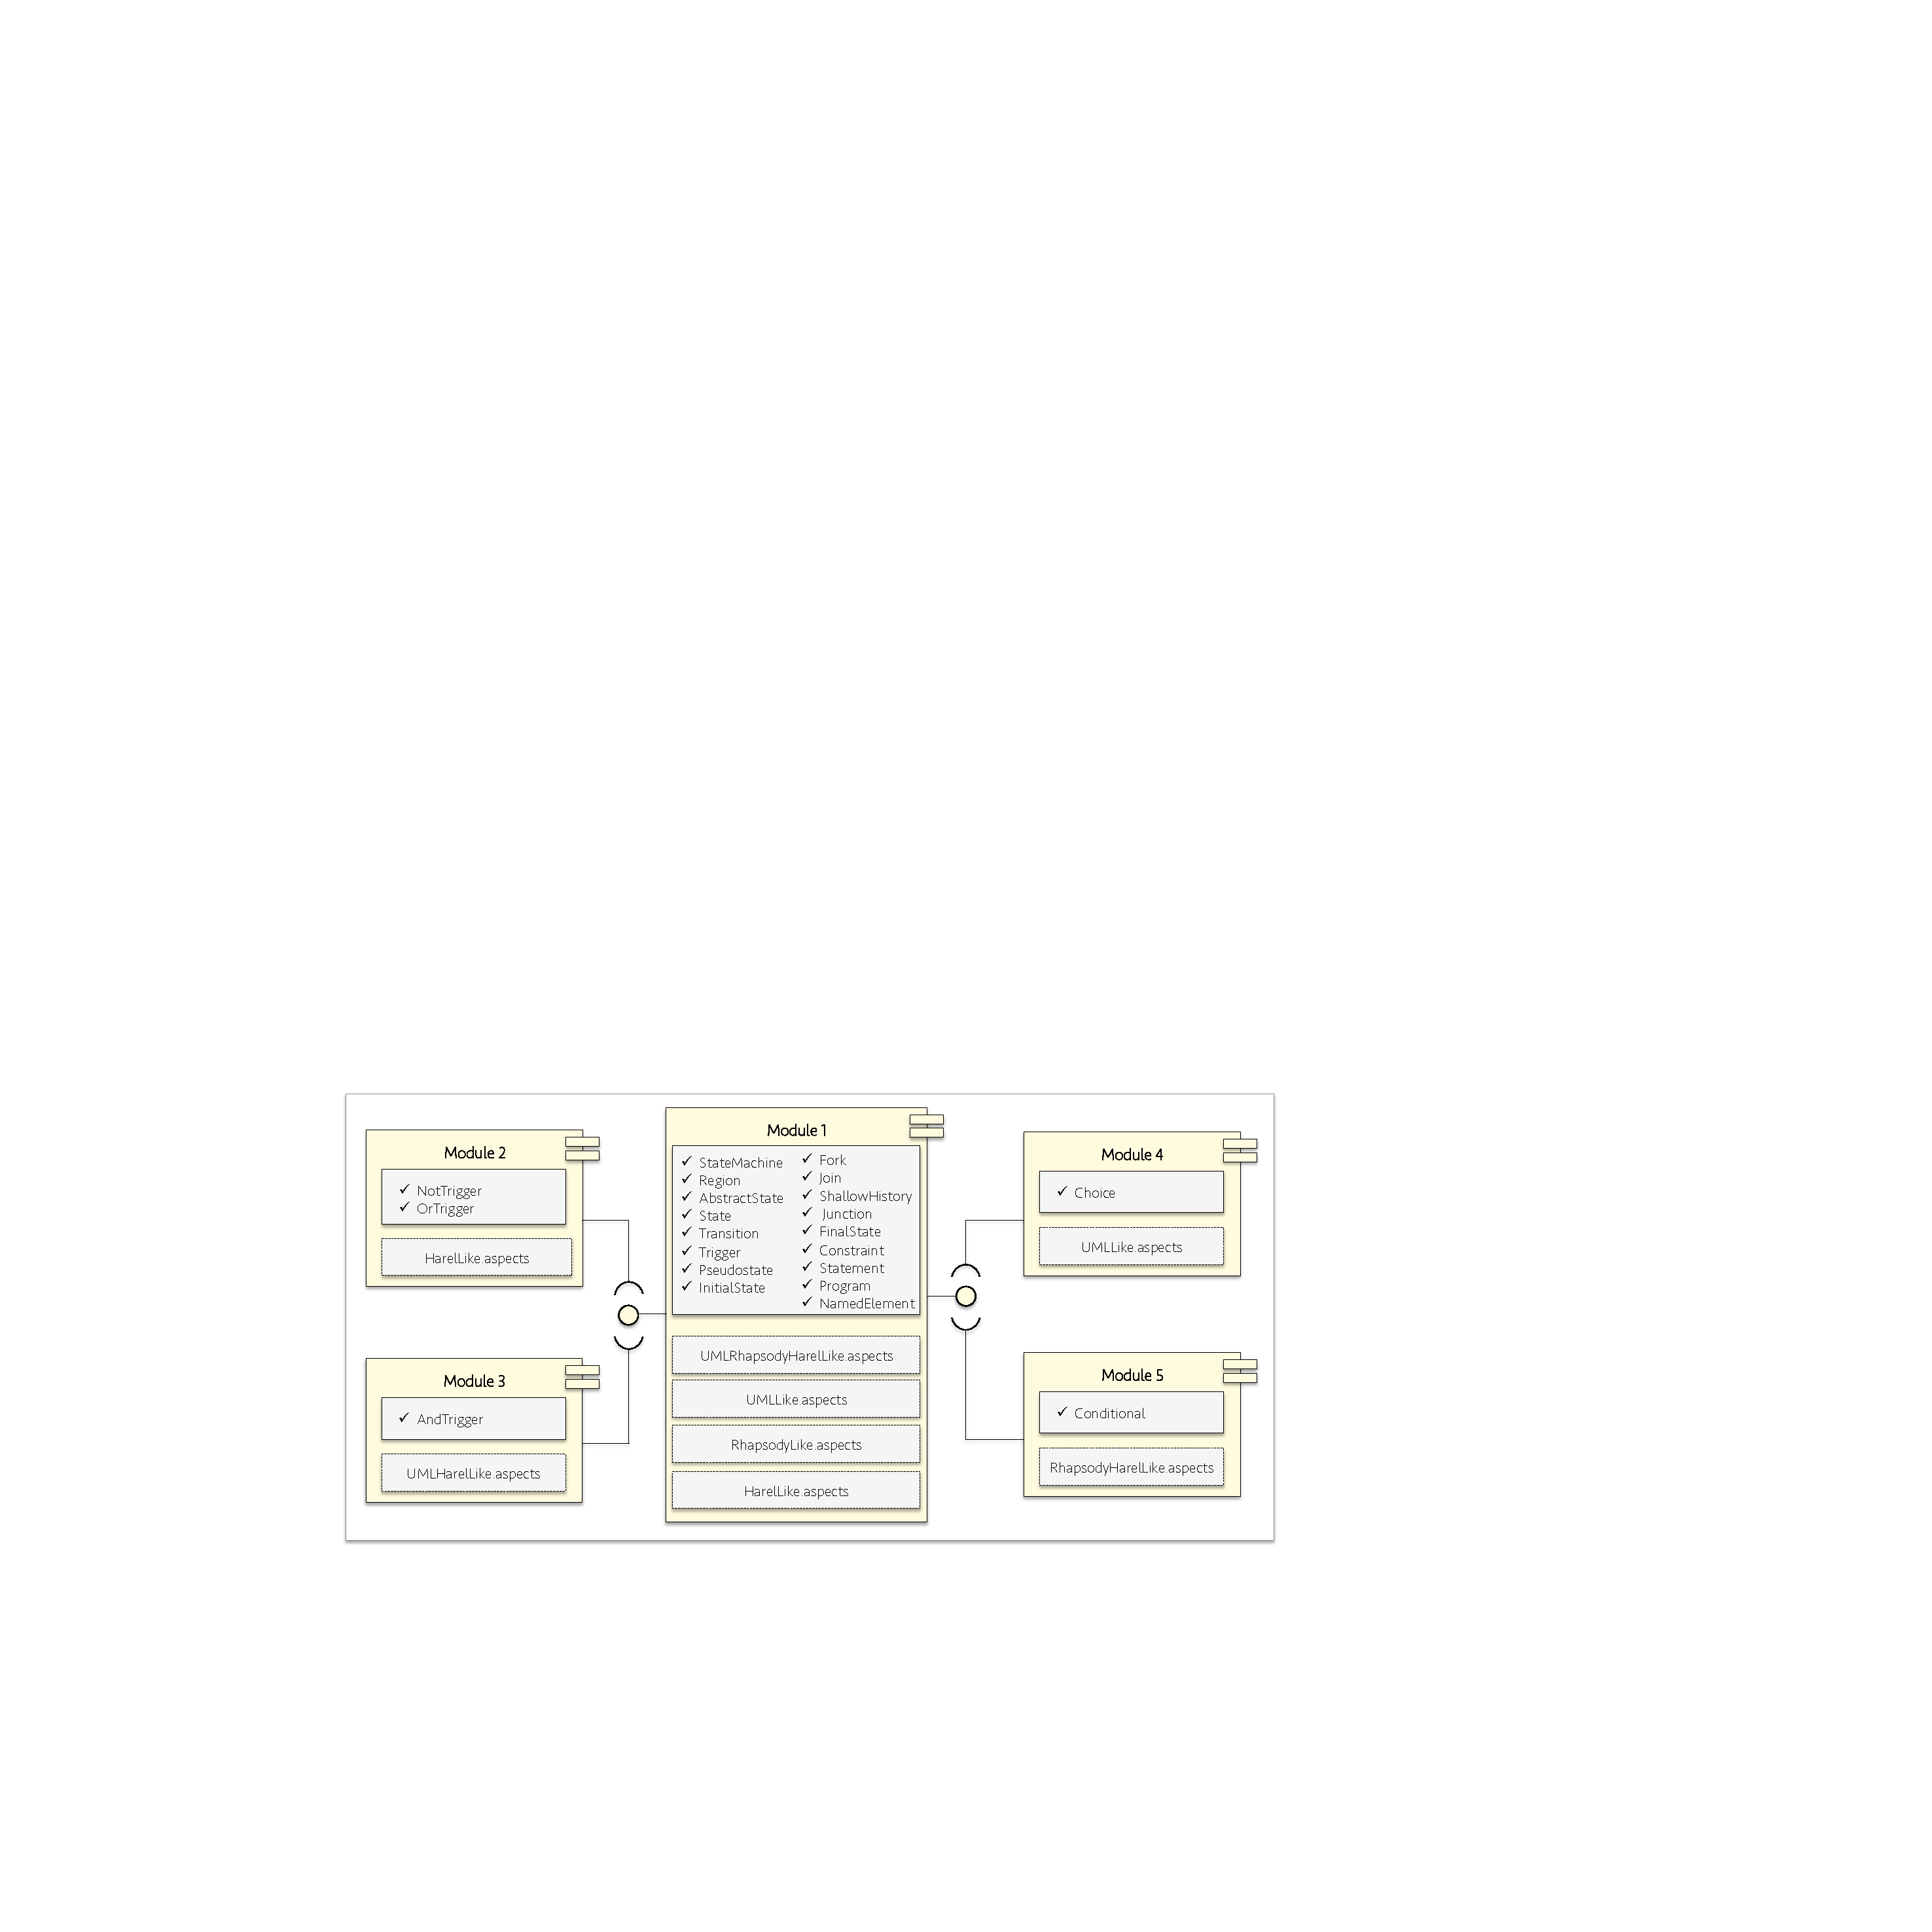
\includegraphics[width=1\linewidth]{images/puzzle-modularization.pdf}
\caption{Results for the state machines case study: extracting language modules}
\label{fig:puzzle-modularization}
\end{figure}

\subsection{Evaluating relevance: Identifying potential reuse in the wild}

The second part of the evaluation of our approach is intended to identify potential reuse in the wild. To do so, we explore the public GitHub repositories and download all the DSLs that fit with the technological space and language workbench we used in our approach. The result of this exploration is a set of metamodels that we can use. However, the semantic part of the DSLs is not that easy since kermeta 3 is a novel approach that is under construction. In any case, we consider that analyzing potential reuse at the level of the syntax is a good insight to know if there is potential reuse.

Once we have the set of metamodels (about 2.800), we build a matrix. 

The experiments were conducted using a version of \toolname implemented in Java. Further, 
\toolname was installed in the Grid5000 Cloud, which is a cluster with more than 5000 cores from were we took XX dual-CPU Dell Blades with Intel Xeon X3470 CPUs running at 2.93GHz, with 16 threads 
per CPU, and CentOS v6. Each dual-CPU Dell Blade has 36GB of RAM. 

%\begin{table*}[htbp]
%  \centering
% \scalebox{0.8}{
%\begin{tabular}{|p{0.2\textwidth}|p{0.3\textwidth}p{0.1\textwidth}p{0.4\textwidth}|}
%\hline
%\multicolumn{4}{|c|}{\textbf{Hypotheses of Experiment 1}} \\ \hline
%\textbf{Null Hypothesis ($H_0$)} & \multicolumn{ 3}{|p{0.8\textwidth}|}{\toolname is capable of detecting %commonalities in the case study that motivated this research.} \\ \hline
%\textbf{Alt. Hypothesis ($H_1$)} & \multicolumn{ 3}{|p{0.8\textwidth}|}{
%\toolname is not capable of detecting commonalities in the case study that motivated this research.} \\ %\hline
%\textbf{Dependent variable} & \multicolumn{ 3}{|p{0.8\textwidth}|}{The set of ecores representing our %languages. }\\ \hline
%\textbf{Blocking variables} & \multicolumn{ 3}{|p{0.8\textwidth}|}{The most sold phones and the market %share indexes. }\\ \hline
%\textbf{Model used as input} & \multicolumn{ 3}{|p{0.8\textwidth}|}{\textit{models in %\url{urlhacialosmodelos}} }
%\\
%\hline \hline


%\multicolumn{4}{|c|}{\textbf{Hypotheses of Experiment 2}} \\ \hline
%\textbf{Null Hypothesis ($H_0$)} & \multicolumn{ 3}{|p{0.8\textwidth}|}{The use of \toolname 
%will not result in a higher market-share impact metric than selecting the most commonly sold 
%phones, for a given maximum budget.} \\ \hline
%\textbf{Alt. Hypothesis ($H_1$)} & \multicolumn{ 3}{|p{0.8\textwidth}|}{The use of \toolname 
%will result in a higher market-share impact metric than selecting the most commonly sold 
%phones, for a given maximum budget.}\\ \hline
%\textbf{Model used as input} & \multicolumn{ 3}{|p{0.8\textwidth}|}{\textit{Android feature model presented %in Figure \ref{fig:featureModel}} }\\ 
%\hline
%% @J - Do you mean independent?! My understanding is that a blocking variable is a grouping variable...
%\textbf{Blocking variables} & \multicolumn{ 3}{|p{0.8\textwidth}|}{The most sold phones, market share %indexes and the maximum cost allowed set to 600\$. }\\ \hline
%\textbf{Model used as input} & \multicolumn{ 3}{|p{0.8\textwidth}|}{\textit{Android feature model presented in Figure \ref{fig:featureModel}} }\\
%\hline \hline

%\multicolumn{4}{|c|}{\textbf{Constants}} \\ \hline
%\textbf{CSP solver} & \multicolumn{ 3}{|p{0.8\textwidth}|}{\textit{ChocoSolver v2} } \\ \hline
%\textbf{Heuristic for variable selection in the CSP solver} & \multicolumn{ 3}{|p{0.8\textwidth}|}{\textit{Default}}\\
%\hline 

%\hline 
%\end{tabular}%
%}
%\caption{Hypotheses and design of experiments.}
%  \label{tab:Exp1aDesign}
%\end{table*}
%\todo{poner la tabla para con los datos de los experimentos que vamos a ejecutar/hemos ejecutado. Intenta pensar cuales pueden ser las conclusiones que quieres extraer. Yo propongo 3 abajo.}

%Table \ref{tab:Exp1aDesign} shows the hypothesis of the experiments executed to validate our 
%approach. To make the experiments reproducible, a number of fixed assumptions are made, such as homogeneous feature costs. ChocoSolver 
%\footnote{\url{http://www.emn.fr/z-info/choco-solver/}}, with it's default heuristic, is 
%used as the CSP solver for extracting software products from the feature model presented 
%in Figure \ref{fig:featureModel}

%\textbf{Technological space and experimental platform:} Currently, there are diverse techniques available for the implementation of syntax and semantics of DSLs \cite{Mernik:2005b}. Language designers can, for example, choose between using context-free grammars or metamodels as specification formalism for syntax. Similarly, there are at least three methods for expressing semantics: operationally, denotationally, and axiomatically \cite{Mosses:2001}. In this paper we are interested on DSLs which syntax is specified by means of metamodels and semantics is specified operationally as a set methods (a.k.a, \textit{domain-specific actions} \cite{Combemale:2013}). Each language construct is specified by means a metaclass and the relationship between language constructs are specified as references between metaclasses. In turn, domain-specific actions are specified as java-like methods that are allocated in each metaclass.
